\documentclass[twoside, 11pt]{scrartcl}

%%%%% General information %%%%%
\title{Overview Over My Bachelor's Thesis}
\author{Jannis Eichborn}

%%%%%%%%%% PACKAGES %%%%%%%%%%%
% basic packages
\usepackage[english]{babel}
\usepackage[utf8]{inputenc}
%\usepackage{cite}
\usepackage[sort]{natbib}
\usepackage{hyperref}
\usepackage{color}
%\usepackage{float}
\usepackage{graphicx}
\usepackage{floatrow}
%\usepackage{showframe}
\usepackage{fancyhdr}

%%%%%%%%%% SETTINGS %%%%%%%%%%%
% No indents, should be unchecked later
%\setlength{\parindent}{0pt}  

% make links in the document interactive
\hypersetup{linktoc=all}
\hypersetup{
    colorlinks,
    citecolor=black,
    filecolor=black,
    linkcolor=black,
    urlcolor=black
}

% Set the style of the header and the footer
\pagestyle{fancy}
\fancyhf{}
\fancyhead[LE,RO]{ }
\fancyhead[RE,LO]{\leftmark}
\fancyfoot[CE,CO]{}
\fancyfoot[RE,LO]{\thepage}
\renewcommand{\headrulewidth}{0.5pt}

% set the style for floating figures
%\floatstyle{boxed}
%\restylefloat{figure}

%%%%%%%%%% NEW FUNCTIONS AND DEFS %%%%%%%%%%%
\def\code#1{\texttt{#1}}

    


%%%%%%%%%%%%%%%%%%%%%%%%%%%%%%%%%%%%%%%%%%%%%%%%%%%%%%%
%%%%%%%%%%%%%%%%%%%%%%%%%%%%%%%%%%%%%%%%%%%%%%%%%%%%%%%
% The actual work
%%%%%%%%%%%%%%%%%%%%%%%%%%%%%%%%%%%%%%%%%%%%%%%%%%%%%%%
%%%%%%%%%%%%%%%%%%%%%%%%%%%%%%%%%%%%%%%%%%%%%%%%%%%%%%%
\begin{document}



\begin{titlepage}
\maketitle
%\textcolor{red}{*Things related to Usability later in the explanations}
\tableofcontents
\end{titlepage}

%%%%%%%%%%%%%%%%%%%%%%%%%%%%%%%%%%%%%%%%%%%%%%%%%%%%%%%
% Introduction
\section{Introduction \& Motivation}
\label{sec:introduction}
%%%%%%%%%%%%%%%%%%%%%%%%%%%%%%%%%%%%%%%%%%%%%%%%%%%%%%%
\subsection{Coding in an Open-Source Environment}

\textbf{Brief Description and History}\\
Here I want to talk about how software is developed, give a brief history on how open-source developed over time and present different approaches of people working together on large problems. \\
What are the main goals of this community and how are these goals expressed?\\

Open Source is one of the biggest buzzwords in the beginning of the 21st century. The way code is developed, the way people work together and the way software is distributed has changed dramatically over the last 15 years. TODO find some kind of source for that!\\

Most of the foundations for Open Source coding were made way earlier. (TODO something about Richard Stolzmann here!). One of the biggest and greatest achievements coming from this community is for example the Unix operating system together with its childen Linux, Debian usw...
These project were huge in terms of time that was put in it, the amount of code produced, the number of collaborators and the spread of usage over the globe (TODO some kind of numbers would be nice for that, also I want to include something which shows the role of the internet in this development, what happened when and where, how were people connected while doing it?).

With the rise of the internet people began to pool their knowledge and skills in ways which were not possible as a couple of years earlier. Programmers began, often in their free time, to input ideas, implementations and critics into open projects which did not earn them any money. Actually very often the licenses used prohibit commercial use of the created programs in any way as does the abundant Apache license TODO LINK.

Why would people do that?
Well there are two often named reasons for that. First of all the free software, where free does not mean gratis but free of commercial interests has a strong ideological background from the people writing and using the programs. It is the belief that if only enough people give to the community it will be self-sustaining and makes everyone actually profit from it. 

Secondly, and I think more recently, people do it for actual credit. They will not be payed for their efforts directly but their efforts and input are visible to many people. You make contacts, generate a reputation and gain credibility which in the end enhances a programmer's chances for better jobs and more interesting challenges.

So the community began to grow quite quickly and it did not take too long until people began to have troubles working together on code. Keeping track of versions, contributions, contributors, bugs, milestones and many more is a challenge already with a couple of people sitting in the same room. Having code written by thousands of developers all over the world then, is a whole different story (TODO find a  source for the development of the linux kernel and the number of contributors).




\textbf{The Open-Source Community is Changing}\\
What are recent developments, how is code shared, where do we want to go?
Which ideals are fulfilled and which  things are still in a messy state?\\

\textbf{What is the Problem with Current Integrated Development Environments?}\\
Introduction of usability in the context of working with IDEs\\
Description of problems in the workflow regarding spreading of code, packages in different forms and finding suitable discussion and documentation. Reuse of code is bad and tedious.


\subsection{Our Idea for Working on Large Projects in the Future}
Description of the idea of having more code in one place with interchangeable and competing solutions. Using crowd sourcing for evaluation...\\
How is the functionality of an online database for code integral part of the IDE's usability?\\

\subsection{My Work \& Goals - A Self-organizing Database for Code}
What exactly will my work do in this context and what are my goals. 
Description of the structure of my thesis. What usability criteria do I aim for?\\

\subsection*{General notes - Abbreviations.}
\begin{itemize}
	\item I will use the term \textit{function} for anything that is a function, method, routine or subroutine in a given language. Maybe just talking about Julia here?
\end{itemize}



%%%%%%%%%%%%%%%%%%%%%%%%%%%%%%%%%%%%%%%%%%%%%%%%%%%%%%%
% Analysis and Formalisation of the Problem
\section{Analysis \& Formalisation}
\label{sec:analysis}
%%%%%%%%%%%%%%%%%%%%%%%%%%%%%%%%%%%%%%%%%%%%%%%%%%%%%%%

\subsection{Description of Use-Cases - Client Requirements}
\label{sec:clientReq}
\textit{This part will include extensive formalisations with respect to usability. How can this be formalised, what metrics can be derived? How do I define the client in this scenario and what is important to this client?\\
I describe how people are going to use the client IDE and what requirements arise from this. I will talk about portability between different OSs, what performance clients want and other aspects which are important to the implementation. What are possible interfaces and how can I meet them?}

% General thoughts
First of all I will have to describe potential clients to my system. What kind of applications will make use of the database, how do they want to communicate and what does this interaction imply for the architecture of the database?

Well to begin with is should be obvious, that I will not be concerned with any kind of graphical interface to the database. It would store millions of entries with several different versions of each entry. Of course one could think of means to make an interactive query interface which can display the database in it entirety but in my mind this is no use case. Users should always query the database in the context of a more elaborate system on top. If you wanted to search for documentation or code only there are already thousands of possibilities to do so on the internet (TODO quote).
From my point of view the system is designed to be used by an IDE or something equivalent. It does not mean that other more 'traditional' use-cases are not possible, but I will not be concerned with those in this chapter. Also the aimed database-representation would probably perform suboptimal for these kind of uses (multiple rapid queries at a time over simple indices). For these tasks there are solutions (TODO quote) out there and they cannot be the target use-cases for my system.

% Example in an IDE
In my mind the focus of the system must be to aggregate over the contained data for more elaborate queries. For example a query in plain English would be something like this: "Give me all the function signatures which match this given set of parameters" or "Which functions have the same parameters and return the same type?".\\
These queries result from using the a possible IDE or smart query system on top of the database. Let me stick with using an IDE for a more extensive example: A User writes a function from the top of his head. He does not refer to anything in the database (yet), but instead simply writes ahead. \\
Right after he has entered the signature the system can check for the following: 
\begin{enumerate}
	\item Is there already a function with the exact \emph{same signature}?\\
Should definitely be shown to the user. Maybe somebody has already done all the work he is going to do now. This might even be an expert in this area who has spend approximately 42 hours upon perfecting the runtime-behavior of this single function. In this case users might be happy to just plug-in the given function as is, or at least make use of the code to get ideas for his own improvements. I think this case might sound pretty uncommon but with thousands of users which roughly confirm to naming-standards of functions, this feature might work pretty fine right out of the box. Also users could then go ahead and write their own variants of this function an re-upload it. This way entering the desired signature alone can be seen as a means to search for functionalities using all the knowledge that you put into the signature.

	\item Is there already a function with the \emph{same name}?\\
Even if the signature is no a match, there might still be quite a lot of use in showing functions which have the same name. They might be different approaches to the same functionality - variations in the parameters might just be due to implementation details - or functions which are similar in their behavior and might need only slight changes to fulfil a new role. As it is the intention to make code reusable and having the database managing all the (sometimes rivalling) code-fragments.

	\item Is there already a function with a very \emph{similar name}?\\
Using some sort of similarity-measure, one could determine a class of function names which are similar enough to the given function name. Best case this is done using the general naming conventions of the language in question. There are two cases that are worthwhile to consider:
	\begin{enumerate}
		\item Are the parameters the same?\\
Then it is most propable that the user will want to see these results. There is quite a lot of information already in the typed parameter to a function. If those correspond it is worth a look to see whether this function might actually what the user wants in this context.
		\item Are the parameters - while not the same - at least similar\\
If the parameters are completely different it will be highly unlikely that the function will do what the user wants to achieve. If however the parameters differ only marginally it might be interesting to see also these function in the database.
	\end{enumerate}
\end{enumerate}

In general this all means that the database must be able to process these kinds of queries with reasonable results for all the given cases. While case 1) seems pretty straightforward, there might be problems when it comes to versioning of code pieces and finding the "best" functions which have the same signature. It is of no use for the user to find himself confronted with more than a dozen nightly-hacked matrix multiplications before the "standard" built-in matrix-multiplication is shown. \\
For all cases in 2) and 3) there is some sort of ranking necessary to present the client with usable results. Also one must consider, that you don't ever want to return \emph{all} results as bandwidth would quickly become a limiting factor to the system, which makes ranking even more interesting.
The system should make use of as much context-information as necessary, even drop down to comments in order to rank functions for a given query.\\

\textbf{Possible queries}
\begin{itemize}
	\item Retrieval of functions:
	\begin{itemize}
		\item Finding matching code to  a signature.(might also include the return type of the function)
		\item Find code to similar signatures or even without a name at all, just so you can see what would be possible with a set of arguments.
		\item Finding matching code to a block of code. (Potentially hazardous)
		\item Retrieving a newer version of code (maybe just the difference)
		\item Retrieving a whole package/module with all functions
		\item Retrieving meta-information to functions. Documentation, connections to other code, dependencies/using/requirements, variations, older version etc... 
		\end{itemize}
	\item Uploading functions:
	\begin{itemize}
		\item A completely new function, without any links. 
		\item Upload an entire module/package
		\item An update/extension to a function which the user wrote
		\item A variant to a function.
		\item Comments to a function
		\item A rating for a function
		\item A connection between code 
	\end{itemize}		
\end{itemize}

	 

\textbf{Defining the desired experience from a client's point of view}
\begin{itemize}
	\item Most obviously: Having a consistent, simple and well documented interface to the database. It is well defined what queries can be made (and how, maybe using DTD) as well as what one can expect as a response to those queries.
	\item The most important criteria: Having fast response times for simple queries (meaning super-fast retrieval of single functions). Searches for larger sets should yield responses quickly as well. Initial guess less than 500ms for first results to arrive.
	\item Finding the most current version of a function
	\item Finding the most relevant function if there are multiple implementations
	\item If one searches for a set of functions or if a query has mutliple matching results, the client will expect some kind of order on the results. This order should feel natural and consistent as people have become used to by modern search engines. If the database fails to deliever at this level people are far less likely to interact with the code and make updates to the system. 
	\item Up to this point I do not want to aim for auto-completion. The client should provide one query and expect a timely answer to it (no streaming yet). Later this feature might get interesting, especially once the database gets partitioned over several clusters and results are aggregated from different sub-graphs. For now my goal will be batched processing of one query after the other.
	\item Having consistent results. The same query deliveres the same answers, similar queries lead to similar results. Priorization should be transparent to a client, or even configurable (using some sort of arguments for a search).
	\item If a client updates information in the database or uploads new content, he will want to get feedback whether this was successful or not. Some auxiliary information might be interesting (what version, where, what size, how long etc...). If the transaction failed for whatever reason the client wants to know why.
\end{itemize}

\textbf{Required funtionalities derived from the desired experience and possible queries}
\begin{itemize}
	\item Fast (indexed) access to the data in various forms:
		\begin{itemize}
			\item function-names (some intelligent search like elastic search to be able to find similar names)
			\item parameters (in combination with the name or without it)
			\item return types in combination with the above.
			\item metainformation (not a priority)
		\end{itemize}		 
	\item Using these finding mechanism the database must be able to return:\
	\begin{itemize}
		\item A whole function, if there is exactly one hit, in a protocolled and serialized manner.
		\item Requested parts of functions (comments, ratings, documentation)
		\item Being able to traverse the graph in order to find connections (versions, similar functions, parameters, usage links etc...). \textbf{This functionalality is very interesting but is also vast and sometimes difficult. Thus it is not a priority.}
	\end{itemize}
	\item Also the database must return sets of functions:
	\begin{itemize}
		\item If a client wants to see/retrieve a package.
		\item If a client searches functions similar to a given signature.
		\item If a client only provides parameters and wants to find matching functions.
	\end{itemize}
\end{itemize}


\subsection{Non-functional (technical) Requirements to the System}
This section focuses on things like scalability, robustness, the iteration speed of changes, whether and where changes to the design are possible and how security and safety standards can or have to be met. Which things are necessary and which ones are nice to have?\\

\textbf{Building an interface}\\
The first task is to provide the functionality of the database-system to a remote client. There must be a suitable protocol in place which can handle the transfer or queries and the responses. Criteria: Quick, secure, fail-safe, well-known and understood. The datastream needed should be minimal to avoid loss of data as well as reducing the time/bandwidth needed for the transactions. A client should be able to use the system without a top-notch internet connection.\\



\textbf{Trying to minimize the time needed for the queries}\\
This is a central requirement.. Making data accessible is what the database is all about. The client-acceptance of the system is dependent on quick response of the system. Having a neat interface (above) is the first step. Furthermore the system must exhibitthe following properties, which I will explain below:
\begin{enumerate}
	\item Consistency of the data in order to keep the amount of space needed for the data minimal.
	\item Monitoring as a means to detect failures and bottlenecks in the system.
	\item Scalability.
	\item Ranking of results.
	\item Feedback when things timeout or fail.
\end{enumerate}


\textbf{1) Consistency of the data}
\begin{itemize}
	\item Being able to produce a \emph{unique} ID for every entry which encodes name, signature and timestamp for the given function which was uploaded. This ID must be unique for every entry but still encode in an understandable manner. A function can be translated to an ID and it must be possible to retrieve a function from an ID. (Indexing or traversals) 
	\item The database needs a valid scheme which represents structures in the data. Since I will use a graph-based system there has to be a graph-representation of the data, which is extendable and concise at the same time in order to prevent overhead in the data-representation while still having the means to extends functionalities in the system.
	\item Items which are put into the database have to be addressable, properly connected and indexed, so that there is no zombie-data in the database. Transactions need to be atomic for retries, dispatchement over different threads and support of thousands of clients. 
	\item One very important aspect is proper versioning of functions. Initially the database should be able to store as many version as the user likes. Over time it could be interesting to implement some garbage collection behavior to sort out unused nodes in the database to prevent the system from becoming overloaded in slow. There must be some way to monitor this behavior.
	\item Having a proper indexing system.
\end{itemize}

\textbf{2) Monitoring}\\
In order to assess the functionality of the database there have to be mechanism to generate and use simple metrics over the system. These metrics can then be used to optimize the behavior of the graph and to evaluate the success of different functionalities. Possible metrics are:
\begin{itemize}
	\item Number of transactions per second.
	\item Overall size of the graph; number of nodes/edges.
	\item Average number of connections between nodes. Distribution of types of connections.
	\item Average number of versions for one function (or other means of central tendency).
	\item How the client-access is distributed, how many calls of what category?
	\item Average times for operations.
	\item Error counts, failure statistics.
\end{itemize}


\textbf{3) Scalability}
\begin{itemize}
	\item The performance of the database must be consistent with growing input. One cannot assume constant behavior but linear would already be pretty bad. Mechanisms must be in place which allow efficient indexing and sorting of data.	
	\item Vertical scalability: If a machine has more resources it should be able to make use of those. More cores mean more threads. Atomic transactions have to be distributed over all available threads using the  provided memory in the heap. That means the database will have to be designed for heavy concurrency in all possible places (reading, writing, garbage collection, metrics).
	\item Horizontal scalability: With more and more data it is vital to be able to partition the data over multiple machines/drives. This should be considered from the start. The database should never be a monolithic process in a single JVM, or at least it must be possible to change that without rewriting the whole codebase. This includes considerations about the consistency of the data over multiple instances or partitions.
\end{itemize}

\textbf{4) Ranking of results} \\
\begin{itemize}
	\item Using some metrics to cap the search-space and the amount of data which has to be retrieved.
	\item This also means not to squander with the number of individual transactions (possibly concurrent) to the database, but to make processing batched. This will help serving a lot of clients while still providing fast answering to every one of them.
	\item There has to be a good understanding of the use-cases and distribution of usage to tune this system. Therefore the initial capabilities will be limited to rudimentary features.
\end{itemize}
  

\subsection{Goals of my Work}
Which derive from the requirements above. Explicit goals with respect to usability.


\subsection{Structure of My Work}
What comes first. How do I want to accomplish the goals and what is the prioritization.


%%%%%%%%%%%%%%%%%%%%%%%%%%%%%%%%%%%%%%%%%%%%%%%%%%%%%%%
% Relevant Basics
\section{Relevant Basics}
\label{sec:basics}
%%%%%%%%%%%%%%%%%%%%%%%%%%%%%%%%%%%%%%%%%%%%%%%%%%%%%%%
\subsection{JVM - Choice of Language and Context}
\label{sec:jvm}
Why it is still relevant in the context of large-scale distributed computation
\subsection{SQL to NoSQL - Why Graph Databases?}
What are recent developments in the requirements on databases and how are those met. New types of databases are emerging.
\subsection{Distributed Databases}
Distributed computations require new forms of data-management. Distributed systems lead to more scalability and robustness in the case of hardware-failures.
\subsection{General Thoughts on Performance \& Scalability in Recent Software Design}
What is the bottleneck in performance nowadays, how is that important to me.

\subsection{Usability in the Context of Technical Systems}
Usability without interfaces. Including thoughts about usability in the structure of a program/package.



%%%%%%%%%%%%%%%%%%%%%%%%%%%%%%%%%%%%%%%%%%%%%%%%%%%%%%%
% Evaluation and Verification
\section{Evaluation \& Verification}
\label{sec:evaluation}
%%%%%%%%%%%%%%%%%%%%%%%%%%%%%%%%%%%%%%%%%%%%%%%%%%%%%%%
\subsection{Why Thinking About Testing Right from the Start Is a Good Idea}
Test-driven design and other thoughts..\\
\textcolor{red}{How do I test for the usability I introduced earlier?}
\subsection{What I Need to Test}
Description of formal aspects which have to be tested. Derivation of suitable measures for the problems.
\subsection{How I Test}
What are the principles in the implementation of my tests.\\
Implementation of usability measures
 

%%%%%%%%%%%%%%%%%%%%%%%%%%%%%%%%%%%%%%%%%%%%%%%%%%%%%%%
% Design and Implementation
\section{Design \& Implementation}
\label{sec:implementation}
%%%%%%%%%%%%%%%%%%%%%%%%%%%%%%%%%%%%%%%%%%%%%%%%%%%%%%%
\subsection{Used Software Packages and Tools}
\label{sec:softwarePackages}
Java has been around for nearly 20 years \cite{link:javaRelease1} and with it came the evolution of the Java Virtual Machine (JVM). As described in section \ref{sec:jvm} there were plenty of reasons for me to make use of the JVM throughout the design of my software.
As I chose Scala as my programming language for the project, I can still make use of any JVM-based package which is very convenient on the one hand but on the other hand also leaves an intimidatingly huge set of possible tools to implement the desired behavior. In this chapter I will name the tools I chose and will explain why with respect to the goals and specifications stated earlier.

\subsubsection{Scala - Choice of Language} % TODO maybe this is better located in the choice of language paragraph in basics
Since Scala compiles into Java-Bytecode it can be seen as a direct surrogate for using Java. The programmer is free to include Java packages and dependencies and one can even use plain Java-code if desired. There were reasons for me to choose Scala over Java:\\

\textbf{Scala is more than Java}\\
Scala was developed from 2001 on and saw its first release in 2003. Martin Odersky was also involved in developing the \textit{Pizza} programming language, the javac compiler and Java Generics in the late 90's which influenced the creation of Scala \cite{link:scalaHistory}.
The resulting language is a hybrid of functional programming elements and object oriented software design. In my personal opinion the simplification of code and the reduction for boilerplate code using functional paradigms is a general trend in the last years and will continue to become more important. Java 8 will include the use of lambda comprehensions and Apple just introduced its new programming language called \textit{Swift} which builds upon Objective-C and includes features derived from functional paradigms to make code more concise and comprehensible. 
As it seems more purely functional programming languages, such as Haskell or Curry, did not yet prove their usability in a production context and are still way off from the object oriented languages such as C, Java and Objective-C which make up the first three entries in the TIOBE software index \cite{link:tiobeIndex}.
In the mentioned index Scala is still way back (place 35) but the point is that general interest in including more functional paradigms into languages exists such as in the high demand of C\#, JavaScript or Python which all exhibit elements of functional programming mostly to make the code more concise and enabling efficient coding in a readable manner.\\
With these developments in the back of your mind I think it is more desirable than ever to harness the power of functional programming because the future points in this direction and many of the smartest minds focus on the reasonable incorporation of functional elements into daily coding.\\

\textbf{Why functional programming is of interest to me}\\
As the supervisor of an internship I have done put it "Scala reduces the amount of code written by roughly 30\%. Thirty percent less code results in 30\% less stupid mistakes in my experience. That was the main reason to introduce Scala to the company". Less boilerplate means less copy and paste, less wrong variable use and more focus on the lines of code you actually write.
This of course is a weak argument although it captures some of the benefits of functional programming. As I said you could achieve the very same thing I am writing in plain Java.\\

But there are some aspects which really make Scala handy.\\
First of all there is the concurrency model I use which is Actor-based concurrency. The idea is that there is no globally shared, mutable state but that all state is encapsulated by actors. This paradigm was developed in the Erlang language, which is functional and was incorporated into Scala under the name of Akka \ref{sec:akka}. Scala feels much more native to this concept since good style in Scala means immutable variables and local scopes rather than global sharing of state.

The rich functional toolset of the Scala collections makes data-transformations, which are needed in most steps of my program, very intuitive and also efficient from a computational point of view. Let me give an example for that: Say you want to take an incoming String from an input to the system which represents an XML and parse all Julia functions contained in it, then check the database if this function already exists and create or update it respectively.

\begin{verbatim}
for {
  function <- juliaParsing.parseFunctionsFromXml(xmlString)
} {
  Database.findFunctionBySignature(function.signature) match {
    case Some(f) => //update the data
    case None    => //create new entry
  }
}
\end{verbatim}

The for-comprehension iterates over all the retrieved functions of let's say type \code{Function} without worrying about the specific type of the result, as long as it is an \code{Iterable$<$Function$>$}. The \code{findFunctionBySignature} method then retrieves the functions if there are any in the database. The result can then be pattern matched to implement the desired behavior. Variables are tightly scoped in this construct and can be efficiently garbage collected after use. The \code{function} variable is very transient yet requires no mutably declared temporary variables.
For comprehensions over the collections in Scala work monadically and are optimized by the compiler which also makes them fast on runtime. Constructs like the one above do appear often in my system for retrieval of data and from my point of view the presented piece of code implements the desired behavior quite elegantly. It also capsules the absence of data without the need for any kind of exceptions by explicitly modeling absence of data. Constructs like these make Scala so appealing to me and in my mind also lead to code which is better readable for other people. My experience is that writing in Scala lets me focus more on the logics behind my transformations rather than looking up API's all day. I also found it easy to read myself into complex systems in Scala.

\subsubsection{Akka}
\label{sec:akka}
Akka \citep{link:akkaHome} is a concurrency-toolkit which is based on the Erlang concurrency model of \textit{Actors} \cite{link:erlangConcurrency}.
The principal idea is that shared mutable state leads to a lot of problems in a multithreaded context. First of all the shared variables have to be locked or mutexed to prevent dirty reads or writes or even data corruption. This blocking behavior means that threads will be idling while they wait for their turn to access the locked variable. It also includes the introduction of boilerplate code to check for the lock and waiting behavior. Also this design is normally not intuitive for a programmer and means adapting to the mindset of a machine rather than having a model which can map a human understanding of parallelism on the machine in an efficient manner.

At the base of the construct is the actor-system in which all the actors live. It comprises a hierarchical structure of actors with their respective children. Thus each actor has a supervisor or parent that decides what to do when an actor crashes and a mailbox which is the only means to communicate with it. An actor is not equal to a thread although it can be implemented that each actor lives on a single thread (which is not recommended, though).
This makes actors totally asynchronous and non-blocking since they will encapsulate their behavior and state, carry out their task when given processor-time and send a message with the result of the computation to another actor. So an actor implements behavior which is triggered by incoming messages, the output is generated by outgoing messages. In Scala these messages can be any kind of class which means there is no boxing needed for transportation between actors.\\

I want to give a very simple example on how this model works:\\
Say we want to do an everyday task also related to my work at hand: \textit{Distributing incoming work from a port}.

\begin{figure}[h]		
 	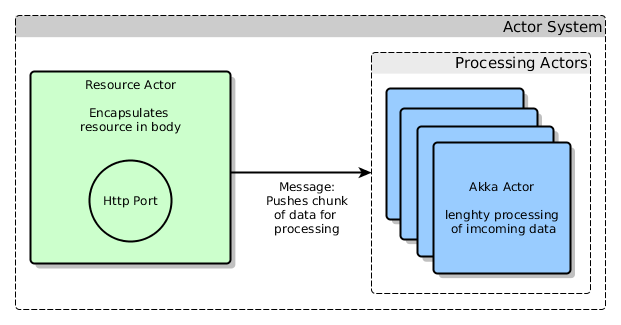
\includegraphics[scale=0.4]{figures/akkaExample1.png}
	\caption{Simple arrangements of actors}
	\label{fig:akkaExample1}
\end{figure}

As seen in figure \ref{fig:akkaExample1} the resource is encapsulated by an actor and not directly accessible from the outside anymore. The Resource actor has sole access to the resource and internally buffers data. The actors which want to process the incoming data need to be known to the Resource so that it can push the incoming work to the processing actors. The source actor will try to find a free actor for the input and then send a message containing the data to it. If there is no free worker, it will buffer the data. I am deliberately leaving out lots of details which would be needed for a functioning implementation, this is just a demonstration of the design principles used.

Already here some things become visible: Actors will not block a thread when there is no work to be done. Only when the source distributes work, the workers will come alive and start doing things, instead of busy waiting or blocking on the source. This is how the system becomes more event-driven which makes a lot of sense in an application that is dependent on input from outside clients.

Failure is another important aspect of an actor system. Let one task in a worker crash due to an unexpected error in the processing of the data, i.e. an error while parsing a data-structure from the input String. One principle of Akka concurrency is not to care too much about all possible exceptions but just to let the actor crash. If this happens it will send a termination message containing the error to its parent and/or supervising actor. 
The supervisor can then decide whether the actor should just continue working using the next message in its mailbox, be restarted, or stopped altogether.
In Akka (and Erlang) this is called the \textit{Error Kernel Pattern} which means that delicate tasks which might crash are delegated to disposable actors which carry no crucial data.

Now for the example the processing actors could be supervised by the source itself, which could decide what to do if one actor crashes. Or this role could be assigned to a designated supervisor actor so that the source and the processing workers live independently, where the supervisor with its children could represent something like a threadpool (See figure \ref{fig:akkaExample2}).

\begin{figure}[h]		
 	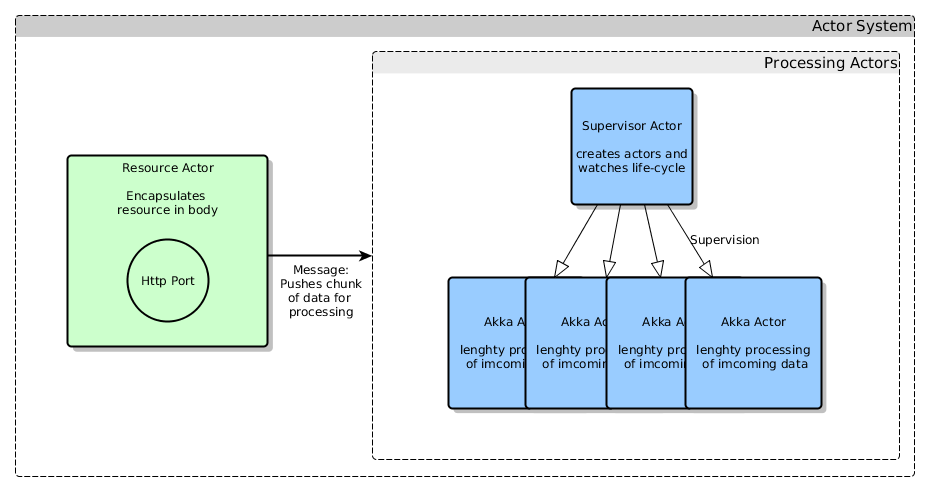
\includegraphics[scale=0.4]{figures/akkaExample2.png}
	\caption{Arrangement of actors with supervision}
	\label{fig:akkaExample2}
\end{figure}

This very flexible model for concurrency allows for the modeling of complex data-flows in large systems. Using supervision and messaging most software patterns such as producer/consumer scenarios or divide and conquer can be implemented elegantly without race conditions, busy waiting, or excessive spawning of threads. Akka has shown some impressive examples on how to run large-scala systems. In fall 2013 they ran a cluster of 2400 nodes on Google Compute Engine which shows how well scaling out via remoting is possible \cite{link:akkaCluster}. Also it is possible to scale up quite drastically. One benchmark shows how a single machine - although an immensely powerful one with 48 cores and 128GB RAM (one of the biggest Amazon EC2 machines, the r3.4xlarge, has 16 cores and 122GB RAM) \cite{link:ec2Pricing} - throughputs around 50 million messages a second in a tuned out system. \cite{link:akkaScaleUp}

I have already worked quite a bit with Akka and am quite pleased with how fast I was able to learn the basics and scale out systems without having to refactor the whole code I wrote for testing. It is easy though to write actor-based code which is quite hard to read since computations happen all throughout the code. A code factoring and a clear documentation seem of outmost importance to me.

Akka is - all in all - a very powerful and flexible tool which provides the possibility to scale in all dimensions. It is a complex tool though with quite some overhead in the implementation. Once this is overcome though, it is an excellent tool to scale a system without having to restructure the code too much.


\subsubsection{Spray}
The Spray toolkit has been developed since 2011 \cite{link:sprayChangelog} and has more than 50 contributors so far \cite{link:sprayGithub}. Their prescribed goal was to create a powerful, flexible and fast HTTP-Server for Scala which works well with other packages and applications and follows good practices for Scala code which have developed so far.

I found this package while I was thinking about how to expose the system to the outside world and began to write Akka-code which has an actor sitting on top of the port, buffering input and flexibly distributing workload over all available processing workers (see the example figure \ref{fig:akkaExample2}). I quickly found out that this would be quite a big task on its own so I started to search for packages which had already done the work for me because I figured that there would be toolkits out there for such a frequently used task. 

First there is the notorious Play framework which is developed in close contact to Akka in the Typesafe Stack \cite{link:play}. 
It offers the developer a complete HTTP server in which you simply route requests. As this sounded promising I took a deeper look into the framework. Soon it became clear that Play is far too optimized for RESTful web-apps which are made to be read by humans. For example it does not offer you too many options to decide on how exactly incoming requests are dispatched to your Akka actor system. The design-focus on REST also means some work-around for my application which quickly begin to make the simple design overwhelmed. The idea of plugging it to an existing actor-system did not appeal to me and I chose to do further search.

My next hit Akka-Spray is in principle exactly what I wanted and even uses the same design principle I have had in mind on how to design the system around the HTTP port.

Fundamentally Spray is built on top of Akka (as is Play) to provide largely parallel, non-blocking and resilient web-applications. It takes away lots of HTTP-tasks from you and lets you focus on implementing on the design of how to multitask your system. However in contrast to Play it does not give you all the overhead of a full blown application but can be seen more as a toolkit which can be used in your already existing program.
It is more complex to use, though. Reasons to still use it were that I already use Akka in other parts of my system which means no more dependencies are added by the system. My intuition was that at one point I would need the flexibility and doing it right from the beginning seemed like a good idea to me here.

Spray handles all incoming requests and boxes them in case classes. The user has to implement how to and where to distribute the incoming requests to actors. This feature was especially important to me. After that it is easy to have actors do the actual work and send back the result, which will then be formatted in a HTTP response.  It will respond with more or less meaningful error messages on things you do not implement and handle time-out strategies for you, which is nice as well.

Since Spray if fully configurable and builds atop of Akka my guess is that scaling of this part of the system is quite unproblematic. 

\subsubsection{Blueprints-API}
Coming to more detailed explanations on which database-system was used I first want to explain the framework which I found to enable a flexible integration of the database to the system.
Actually this was the starting point of my work and is in my mind the most interesting part regarding the software used, since everything I do circles around having a database which enables the functionalities in mind (see \cite{link:blueprints} for more information).
The idea of Blueprints is to provide a complete hierarchy of classes and interfaces to support multiple underlying databases without the need to change your higher-level code. This seemed like a perfect fit for me since my system has the low-level code area which is the database but on the other hand the is the higher-level code segments in the actor system up to the HTTP connection which is supposed to be independent from the underlying database.
There are many implementations of the Blueprints API including the MongoDB based MongoDBGraph an OrientDB implementation called OrientDBGraph and Titan Graph database.
In the end Blueprint lets me choose exactly the desired level of abstraction for my application and nicely frames many things happening with the database. It makes it easy to build a loosely coupled application where parts can be interchangeable without having to rewrite large amounts of other code.
The API also offers supplementary utilities for graphs such as a toolkit for algorithms (Furnace), an DSL for traversals (Gremlin) and tools for dataflow processing (Pipes).


\subsubsection{Titan Database}
Titan Database is an implementation of the Blueprints interface developed since 2012 and builds the functionality of a graph database using variable backends. It promises easy scalability, complex graph traversals, ACID and eventual consistency and seamless integration of indexing backends, namely Elastic Search and Apache Lucene (s.o. \cite{link:titanHome} for further information).

Supported backends include Cassandra, HBase and most interestingly Oracle Berkeley DB. The latter was of interest since it allows for fast prototyping in memory without having to handle a large database in which keys have to be created, dropped and recreated when things change \cite{link:berkeleyDB} As a playground it is perfect and actually in itself already quite capable as it can accommodate 10-100 million vertices on normal machines \cite{link:titanWithBerkeley}.

The ability to change the backend and connecting to existing databases is a useful feature in my mind. I can do prototyping with one kind of database and then switch to another one with changes mostly done in configuration. This could also mean that the database  could eventually live on another machine altogether. Together with Blueprint's abilities this ensures that I can build prototypes quickly yet still write code which can actually be used for bigger systems later without many changes in the logic of the code. It helps designing a system with headroom in the backend without having to do major refactoring to scale the system up or out. Also the user can plugin different indexing backends which comes in handy for me, as well.

Titan makes full use of the Blueprints syntax to iterate over the graph and thus enables a rich existing toolkit to be used.

\subsubsection{Elastic Search}
Last but not least I want to introduce Elastic Search to the system as an indexing-backend. Indexing in my graph database will be important since nodes are normally retrieved using parent nodes and descending in the graph. For example if one wants to find a function with a specific name the system would go to the general function node and iterate over all children-nodes. This is a linear operation which can be quite costly once the system becomes loaded and introduces a large toll on the most important task: searching the database for functions and their implementations. Thus indexing can be used over keys to allow fast access of elements. Later the indices could also be used to power a search-engine for parts of text in the documentation or parts of source-code itself.
Elastic search is open source and was founded in 2012 and has since seen dramatic growth. Just recently it received a \$70 million round C-funding while having around half a million downloads of their software a month. \cite{link:esAbout} \cite{link:esTechCrunch} I have seen it in use in big-data contexts to power meaningful search over largely unstructured data in near real-time. The indices generated could even be used to monitor performance in the system such as frequencies of transactions, update-times, number of users and many more in real-time. I wanted to introduce Elastic Search right from the beginning because of the huge potential in usages later and because the initial overhead is very small.

It is a powerful tool to create queryable indices on a multitude of data sources. It allows for quick context dependent search, completion and scoping of queries and fast access to elements in the database.
Some applications which use Elastic Search on a big scale include Github, SoundCloud and Yelp!. These companies use the software over terrabytes of data and billions of datapoints. \cite{link:esUses}
	
\subsection{First Sketch - Design of my Implementation}
\label{sec:firstSketch}

\begin{figure}[h!]		
 	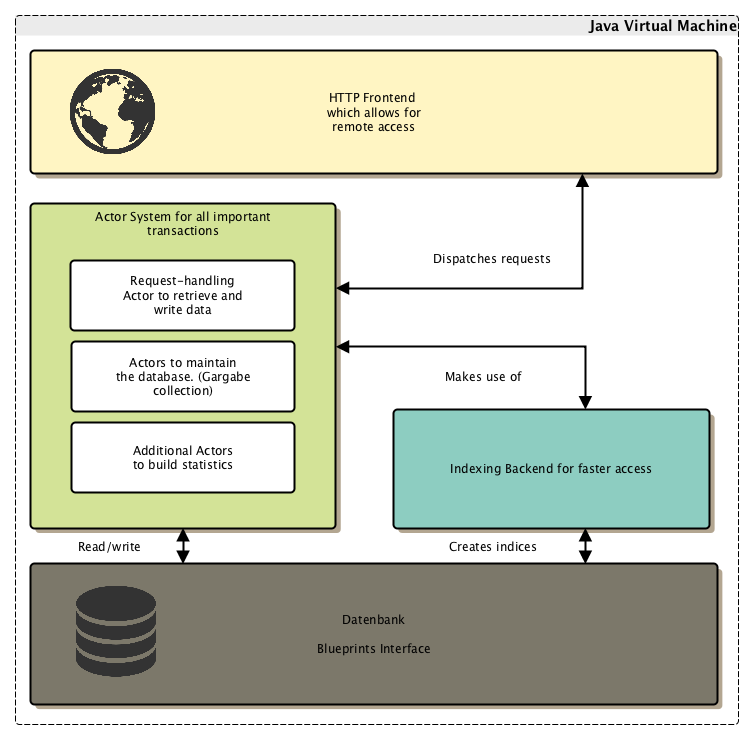
\includegraphics[scale=0.5]{figures/roughOverview.png}
	\caption{Overview over the system}
	\label{fig:roughOverview}
\end{figure}

\subsubsection{Elements of the Design}
% Rough overview
Having all the tools mentioned in \ref{sec:softwarePackages} my initial design sketch has several parts to consider as seen in figure \ref{fig:roughOverview}
\begin{enumerate}
	\item The Database in which data are stored and retrieved from.
	\item An indexing backend which reads the database and creates the indices for fast access.
	\item A system of Akka-actors which can work on the database in serveral ways:
	\begin{enumerate}
		\item To write and retrieve things to and from the database.
		\item Actors to maintain the database
		\item To build statistics on the available data.		
	\end{enumerate}	
	\item An HTTP 'frontend' which offers the handles to the functionality of the database to the outside world.
\end{enumerate}

A general principle for the first sketch is to run as much as possible in the same JVM to enhance inner-process speed and make the configuration more straightforward by not having several different settings for all the different parts of the system. This also speeds up the startup procedure and centralizes logging for faster analysis when things go wrong. \\

\textbf{1. The Database}\\
For the first prototype I chose the backend to be a Titan Database configured for decent parallel access. As a storage backend the first prototype has a BerkeleyDB in-memory database which keeps the data used for queries on the heap which of course will only work for rather small databases. But it is easy to setup and actually works quite well on home-sized machines. My testing-server is a low-energy optimized machine with a tiny dual-core processor so having things in memory will definitely help having moderate testing performance. As stated in the Titan Documentation (\cite{link:titanWithBerkeley}) this database can already hold a couple million nodes and edges and is thus sufficient for the early testing of storing schemes. 
The database itself already allows for parallel access. I simply use this database without any changes to the interface, all this will happen on the level of actors later. I tried to change as little as possible and do next to nothing in terms of optimization of this database. "Premature optimization is the root of all evil", as a popular saying has it \cite{quote:rootEvil}. The plan is to do a bare-bone running version, run the tests and based on those decide where bottlenecks are to be found.
In principle everything which runs on this database is applicable to any of the Titan-Database-backends without any actual changes to the code at all. The only thing which might change are settings in the configuration for the application to allow connection to the remote JVM which runs the database.
Building on this foundation should allow for meaningful tests which can give good predictions of the performance of a more elaborate setup.\\

\textbf{2. The Indexing Backend}\\
This is actually very straightforward because Elastic Search can be embedded into the Berkeley Database with the disadvantage, that it will only be accessible from the same JVM. For the first prototype this does not cause problems since I want to run everything in the same virtual machine anyways. 
The indices have to be created when keys are introduced to the database to allow for fast incremental indexing. I index over the name of nodes 

TODO LIST over what I plan to index and how this index can be used for faster retrieval and/or search.	\\

\textbf{3. The Actor System to Do the Processing}\\	
The single most important and interesting part of the system is the Akka actor system with its various functions for the database. This is the part where the online system really begins to come alive since it offers the processing powers to enhance the system over the functionality of a simple remotely accessed database or a version control system. 
Initially there are three functions a)-c) to be distinguished:\\

a)A set of actors which exist to process incoming requests from \textit{users} of the database. \\

I want this level of the program to abstract away from different databases and their details in implementation, so that the frontend does not need to care about the database used.
So in principle there is an architecture of classes for the actors in place which means that only the lowest level of actors has to adapt to the details of the database implementation used. General functionality such as supervision, behavior on timeout, handling of wrong queries and the communication with the frontend is handled higher up in the architecture to whatever extend this can be implemented.
This has some interesting effects:
Behavior of the system can be tested and reasoned over on a higher level, boilerplate code is minimized and actors become interchangeable depending on the backend which is in place. This means that potentially, actors could be switched \textit{on runtime} to adapt to situations in the system. For example there could be one actor which handles reads and writes but when the database is overloaded, actors will be put in place which refuse to do some computationally expensive tasks. Having this structure allows for very fine-grained control over the handling of requests. Actors can react to small changes themselves but could also be switched altogether when there exist significant problems.
Akka actors are pretty lightweight (since they do not represent a thread) and are thus cheap to create and destruct. In the first implementation I make use of this fact as such that I simply spawn a new worker for every incoming connection to the database. It will then handle all communication from the user to the  backend  and once the connection is shut down it will silently die and release all its resources. Of course this reasoning is based on a hypothetical world where there are no problems with garbage collection in the JVM. My guess is that this might be one of the first bottlenecks in the system. One way to overcome this could be to make use of actor-pools instead of dynamically spawning them and destroying them after (a possibly very) brief lifetime.
As a general design principle one can see the separation of implementation of processing-logics and behavior. An actor implementation should - in my opinion - describe the \textit{what} of connection handling meaning how to connect a user, how to funnel his request to the database, retrieve the results and send them back rather than the \textit{how}. This is why my actors try to carry as little of actual parsing, database or number-crunching code, but rather call static objects which contain the implementation. It is very easy to exchange implementations for different databases without refactoring any of the code used inside the actor. Handling connections is closely connected to the Spray, thus I will explain it in the upcoming paragraph on the frontend.\\

b) Garbage collection in the database\\
In my mind one of the upcoming challenges for the database is cluttering because of the very open structure for writing to the database.
There might be thousands of implementations for one method or a user decided to make unnecessarily many versions of his code.
The database should be able to reduce quantity on some levels. For example it could remove older versions of code which were not used for a very long time, index only recent versions, delete unpopular code or compact things which have not been used for some time.
The idea here is to iterate over parts of the database which were not maintained for some time and iterate over the produced statistics and use decision rules what to remove. The first design will focus only on the most important things and will most likely not incorporate any of the above named.\\

c) Creating statistics on the database\\
This is were I imagine the power of graph databases to really begin to shine. Iterating over existing functions and the collected metrics such as usage counts, usage dates, number of distinct users, number of implementations and many basic metrics more to create meaningful higher level statistics. This could include recommendation of code based on concepts such as code complexity, amount of dependencies, speed, memory-efficiency and so forth. These workers are supposed to work quite similar to the garbage collection in that they can be spawned depending on how much capacity there is (let's say during times where not that many users visit the system) and then do independent runs on subbranches of the database without corrupting the state of other parts. Those workers will have to do quite expensive number crunching  and at this point it has to show how well this can work in the end. In the end these actors will have to work quite close to the database used and at this point an exact scheme of abstraction does not seem helpful.\\

\textbf{4. The Frontend to Open the System to the Outside World}\\
I chose the Spray framework for this task as explained earlier in \ref{sec:softwarePackages}. I want to say something about connecting the HTTP-Server to the actor system and how workload will be dispatched.
First of all what happens in Spray is that the configured port on which the application listens is encapsulated by a dispatching actor. This actor extends a Spray class which does all the nitty gritty details of the HTTP transfer and leaves you to implement where to send the requests to. In principle every incoming request  is quickly forwarded to an actor which functions as a dispatcher, so that the port is free all the time. This dispatcher buffers the imcoming requests and then distributes the workload accordingly. In my case it will take a request and on the fly create a new actor which will process the task at hand. One - I think - very beautiful aspect of Spray is that every actor which takes an incoming request from the dispatcher implicitly knows where to send back the computed response to without seeing any of it in the code. Also the dispatcher knows about the actor processing the request and will send an adequate error message back to the user on failure such as a timeout or a complete crash of an actor. This way error handling becomes quite elegant and effortless since the handling actors do not need to implement any of it in most cases. Their crashing should give enough information to the dispatcher. Once the dispatcher knows about problems in the backend it could change dispatching strategies or dispatch a different kind of handling-actors altogether.

From the point of dispatching a request to a handling actor on everything happens totally asynchronously and non-blockingly. The actor depends on nothing but his own local state, reading or writing from or to the database and then returning the response once it is done working. There is no timing needed, no waiting on things and thus the chance for serious deadlocks or race conditions is pretty low.

One interesting aspect for the first sketch is the fact that I use the actor-system created for Spray for all the actors handling requests to the database. This may be a bit brittle for the long run but does pretty fine in the short run since the actors are created by Spray and are thus "nearby" with no remote handling needed. Also these actors form a necessary unit with the HTTP server. One does not make sense without the other.

\begin{figure}[h!]		
 	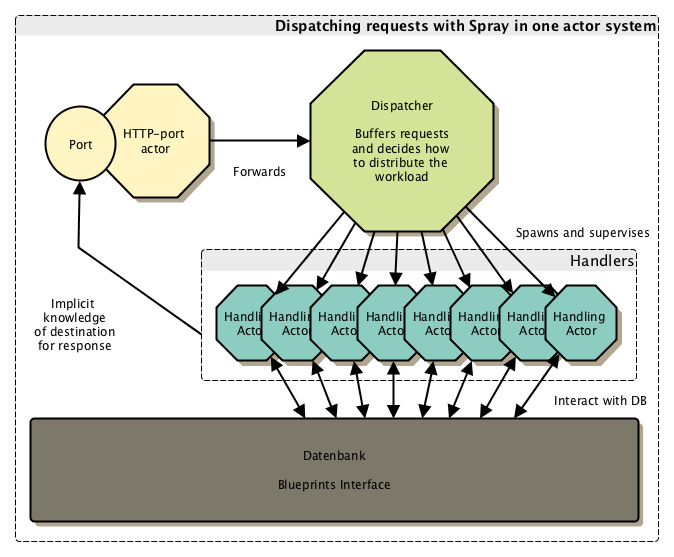
\includegraphics[scale=0.6]{figures/sprayDispatcher.png}
	\caption{How the Dispatcher distributes requests}
	\label{fig:sprayDispatcher}
\end{figure}

\subsubsection{Database Schema}
The term database schema must not be confused with what it means in 'classical' relational databases (as for example in chapter three of \cite{fundamentalsDatabase}). I mean the structure of nodes and edges in combination with fields within the two. Nevertheless this schema must be well thought as well since it will determine what kind of tasks can be accomplished quickly and satisfactory to the user. The schema will be explained exemplary instead of giving an all-engrossing explanation of the schema to show the underlying ideas rather than listing all the details which come with an implementation like this. Also having a graph database means that the structure is best explained by figures instead of text.\\

First of all I want to build a graph which offers different entry points to traverse the graph to extract elements in a meaningful context. Traversals will also be used to create the statistics later on. Figure \ref{fig:dbStructure1} shows how this structure is built for the central storage unit of Julia functions. Most of the tree are meta-nodes which do not contain any code but define the place of the code. The code itself then resides in the leafs (which are a specific version of a method's implementation).  The meta-structure is crucial to the database since this is the part where the graph structure really comes into play separating it from a relational database (which would contain the leafs in tables).

\begin{figure}[h!]		
	\floatbox[{\capbeside\thisfloatsetup{capbesideposition={right,top},capbesidewidth=6cm}}]{figure}[\FBwidth]
	{\caption{The general organization for functions in the database. There is a function node which is parent to all function nodes which represent only names for functions (corresponding to symbols in Julia). Depicted here is one specific Function A with all its subtrees, leaving out all the other possible functions. The children of a function are the multiply dispatched methods which have a unique signature. The next deeper level are different implementations for one method (possibly by different users or focusing on different aspects) and then finally the leafs containing all the code, documentation and other (meta-)data are called version (at different time points). Having this structure alows for traversals to find all methods for a function or any of the version for any of the implementation using straightforward graph-syntax from the Blueprints interface.}\label{fig:dbStructure1}}
	{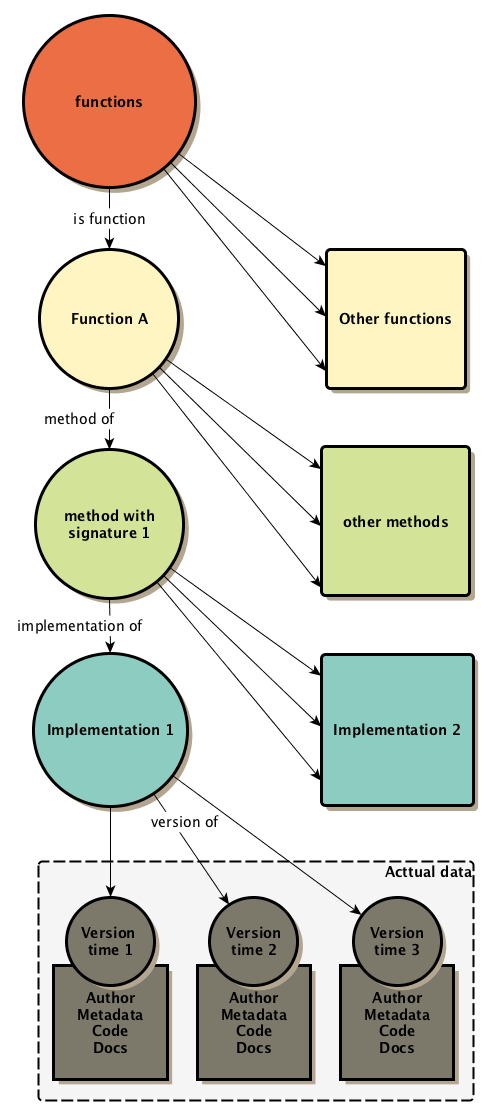
\includegraphics[width=8cm]{figures/dbStructure1}}
\end{figure}

Extending this structure to yield more entry points and possibilities for traversals is depicted in figure \ref{fig:dbStructure2}. Here I introduced structures to link Julia types to where they are used in arguments and introduced a draft to declare dependencies in the graph. Note that this structure does not alter the functions themselves, but just adds more nodes and edges. In reality with Titan Databases it is possible to add structure later on without the need to reload data. This might come in very handy when trying to extend functionality of the system.

\begin{figure}[h!]		
 	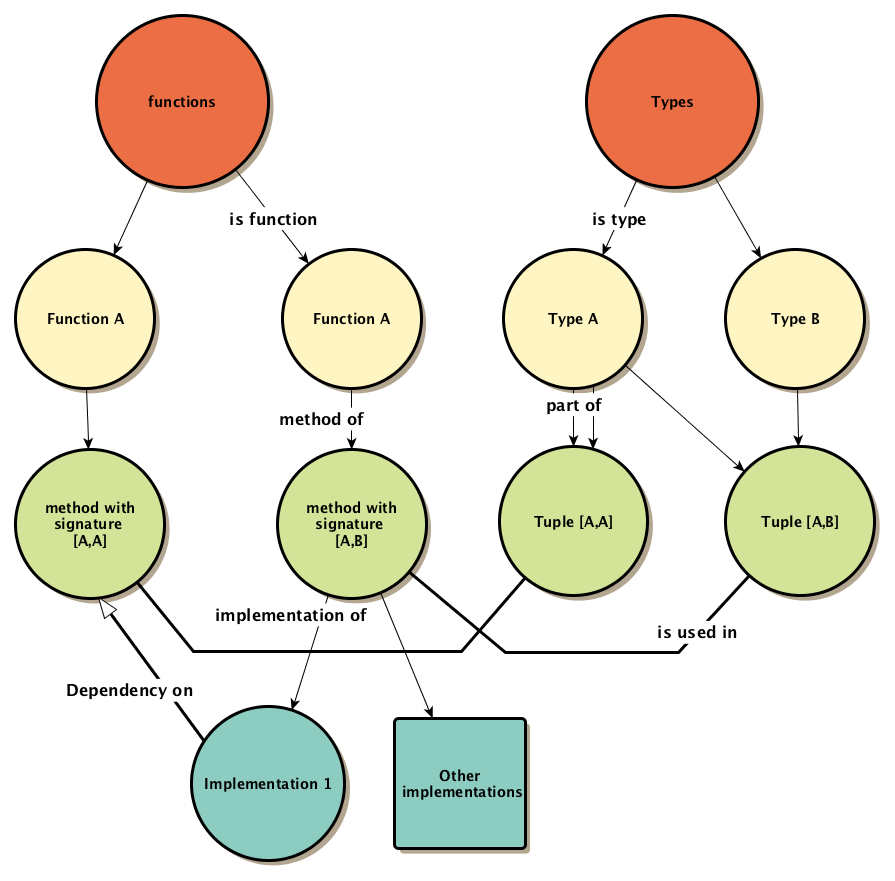
\includegraphics[scale=0.4]{figures/dbStructure2.png}
	\caption{Added structures in the database.}
	\label{fig:dbStructure2}
\end{figure}

Statistical data is incorporated into the meta-structure and the leaf nodes themselves. Usage counts, sets of users, last updates, ratings, complexity, speed or memory consumption and any other metric imaginable can be stored for different methods of functions and also for different implementations of one method.

\subsubsection{The HTTP-Protocol}
Central from a user's point of view is the access to the system. Since I want the program to be client agnostic I chose HTTP as an interface because its structure closely matches the desired functionality of the program. HTTP is supposed to be restful (which is not always the case) which is definitely of good use when modeling a database-connection.

Users can do GET requests to retrieve data, including specifications of parameters in the header and even pieces of code in the body of a request. Insertions into the database can be modeled via POST requests. 

HTTP then offers many error codes when things go wrong. From timing out to temporary unavailability there are lot of messages which are well documented and used in thousands of websites and thus well-known to most programmers who want to create a client to the system.

--- TODO  genaue Struktur erst klar, wenn ein paar Tests gemacht wurden ---



\subsection{A deeper look into the implementation - for those interested}
All actors carry most of the implementation code in their companion object instead of the class itself to decouple implementations of logics from those of behavior. The cake pattern \cite{link:cakePattern} makes it possible to implement much of the connection handling in the trait HandlerActor without any code to handle a database.  An instance of DbHandlerActor is then used with an instance of the trait DbInteractions. This trait mixes in the needed details to connect to a specific database. Using this pattern the system is very flexible to incorporate different databases or changes to implementation without disturbing other parts of the system. To be continued...

\begin{figure}[h!]		
 	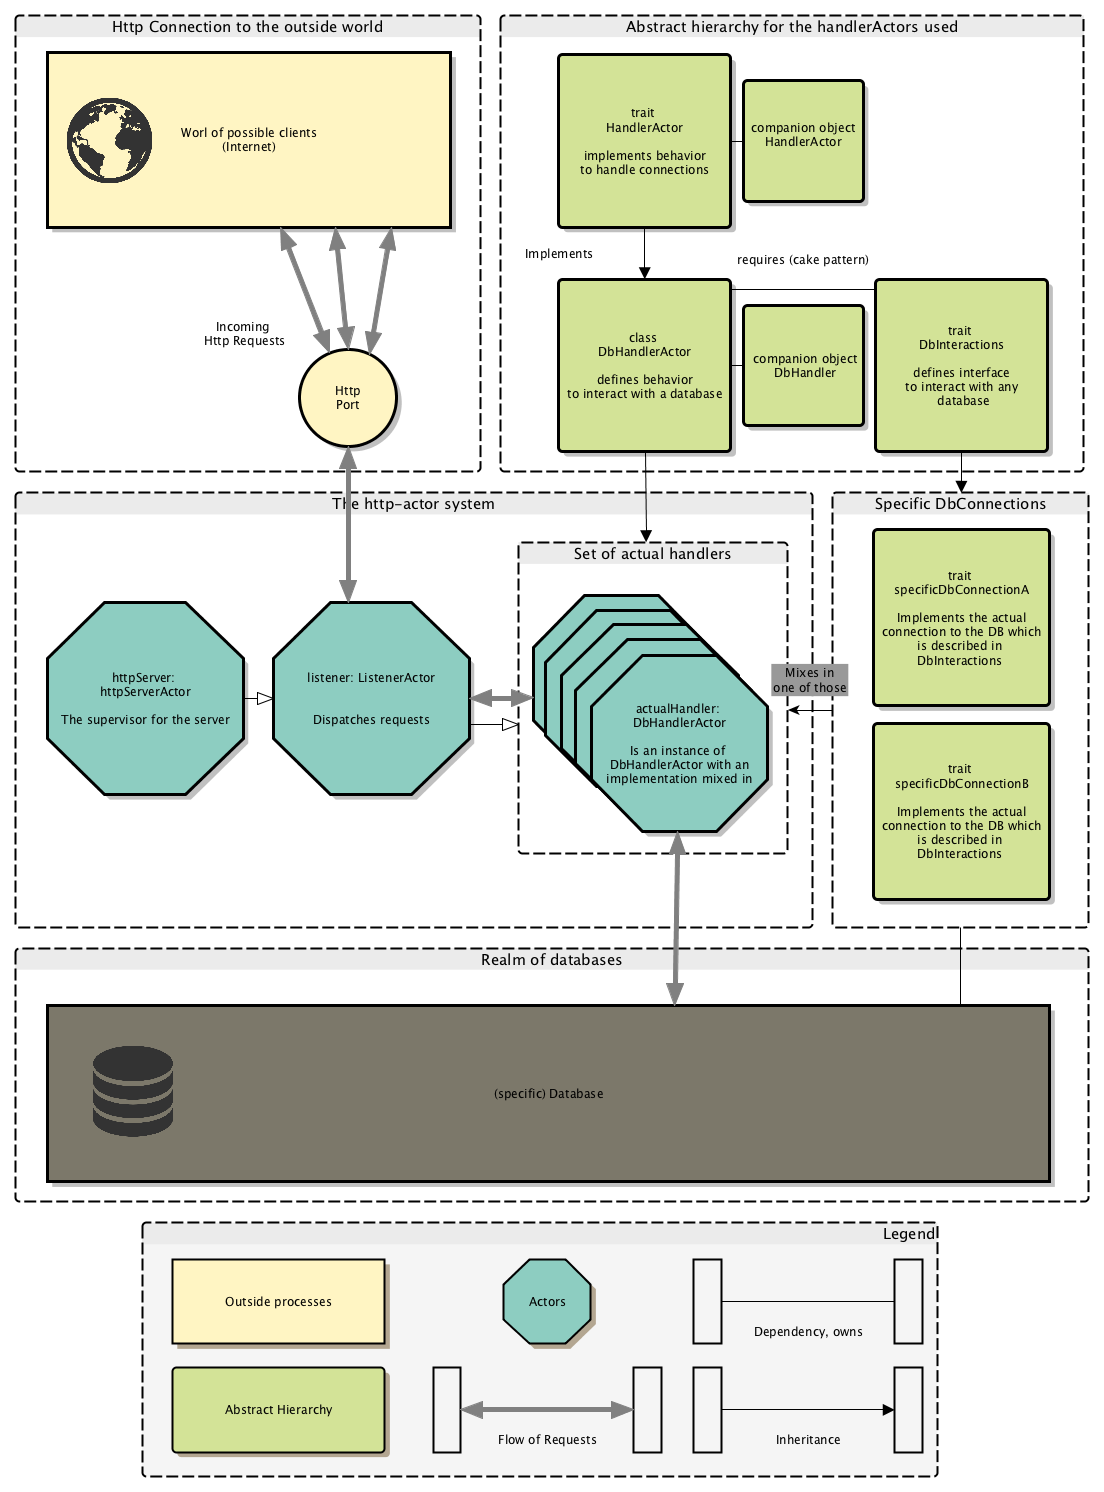
\includegraphics[scale=0.35]{figures/requestFlow.png}
	\caption{Detailed view of the system and how requests are handled. }
	\label{fig:requestFlow}
\end{figure}

\subsection{Evaluation of the First Sketch}
\subsection{Description of the Iteration}
\subsection{Further Evaluation}




%%%%%%%%%%%%%%%%%%%%%%%%%%%%%%%%%%%%%%%%%%%%%%%%%%%%%%%
% Conclusions
\section{Conclusions}
\label{sec:conclusions}
%%%%%%%%%%%%%%%%%%%%%%%%%%%%%%%%%%%%%%%%%%%%%%%%%%%%%%%
\subsection{State of the Implementation at the End of My Work}
\subsection{Comparison to Requirements and Goals}
What was fulfilled, what not and what might be critical. Can the application be extended? What have I achieved at what can people to with it at the time?\\
%\textcolor{red}{Is the code I wrote usable from the clients perspective?}
\subsection{What to Come - Future from here on}
What are the next steps and which people can get involved. How do I see the chances in the future. Concluding thoughts on performance and scalability.
\subsection{Summary}


%%%%%%%%%%%%%%%%%%%%%%%%%%%%%%%%%%%%%%%%%%%%%%%%%%%%%%%
% Appendix
%%%%%%%%%%%%%%%%%%%%%%%%%%%%%%%%%%%%%%%%%%%%%%%%%%%%%%%
\section*{Appendix A - References}
%%%%%%% Bibliographie %%%%%%%%%
\bibliography{sources}
\bibliographystyle{plain}

\end{document}